\documentclass[11pt]{paper}
\usepackage{fullpage}
\usepackage{graphicx}
\usepackage{palatino}
\usepackage{fancyhdr}
\usepackage{draftwatermark}
\usepackage{enumitem}
\setlist{nolistsep}

\renewcommand{\headheight}{0.4in}
\setlength{\headsep}{0.1in}

\setlength{\headwidth}{\textwidth}
\fancyhead[R]{\footnotesize m-labs.hk}
\fancyhead[L]{
   
\includegraphics[height=0.17in]{m_labs_logo.pdf}
}
\chead{}
\rfoot{}
\cfoot{\thepage}
\lfoot{}\pagestyle{fancy}

\begin{document}

\title{The Sinara device family}
\subtitle{high quality hardware for ARTIQ}
\author{S\'ebastien Bourdeauducq, Robert J\"ordens (M-Labs)}

\maketitle

\section{Background and objectives}
Control electronics used in many trapped-ion and other quantum physics experiments suffers from a number of problems. In general, an ad-hoc solution is hastily put together in-house without enough consideration about good design, reproducibility, testing and documentation. This makes those systems unreliable, fragile, and difficult to use and maintain. It also duplicates work in different laboratories. In addition, the performance and features of the existing systems (e.g.\ regarding pulse shaping abilities) is becoming insufficient for some experiments.

To alleviate those problems, M-Labs wish to propose high-quality and turnkey control hardware, which should be in particular:
\begin{itemize}
\item reproducible and open
\item flexible and modular
\item well tested
\item well supported by the ARTIQ control software
\end{itemize}

This document describes the desired components and features of this system.

We thank Joe Britton (ARL), Grzegorz Kasprowicz (Creotech/Warsaw University of Technology), David Leibrandt (NIST), and Daniel Slichter (NIST) for their valuable input.

\section{System overview}

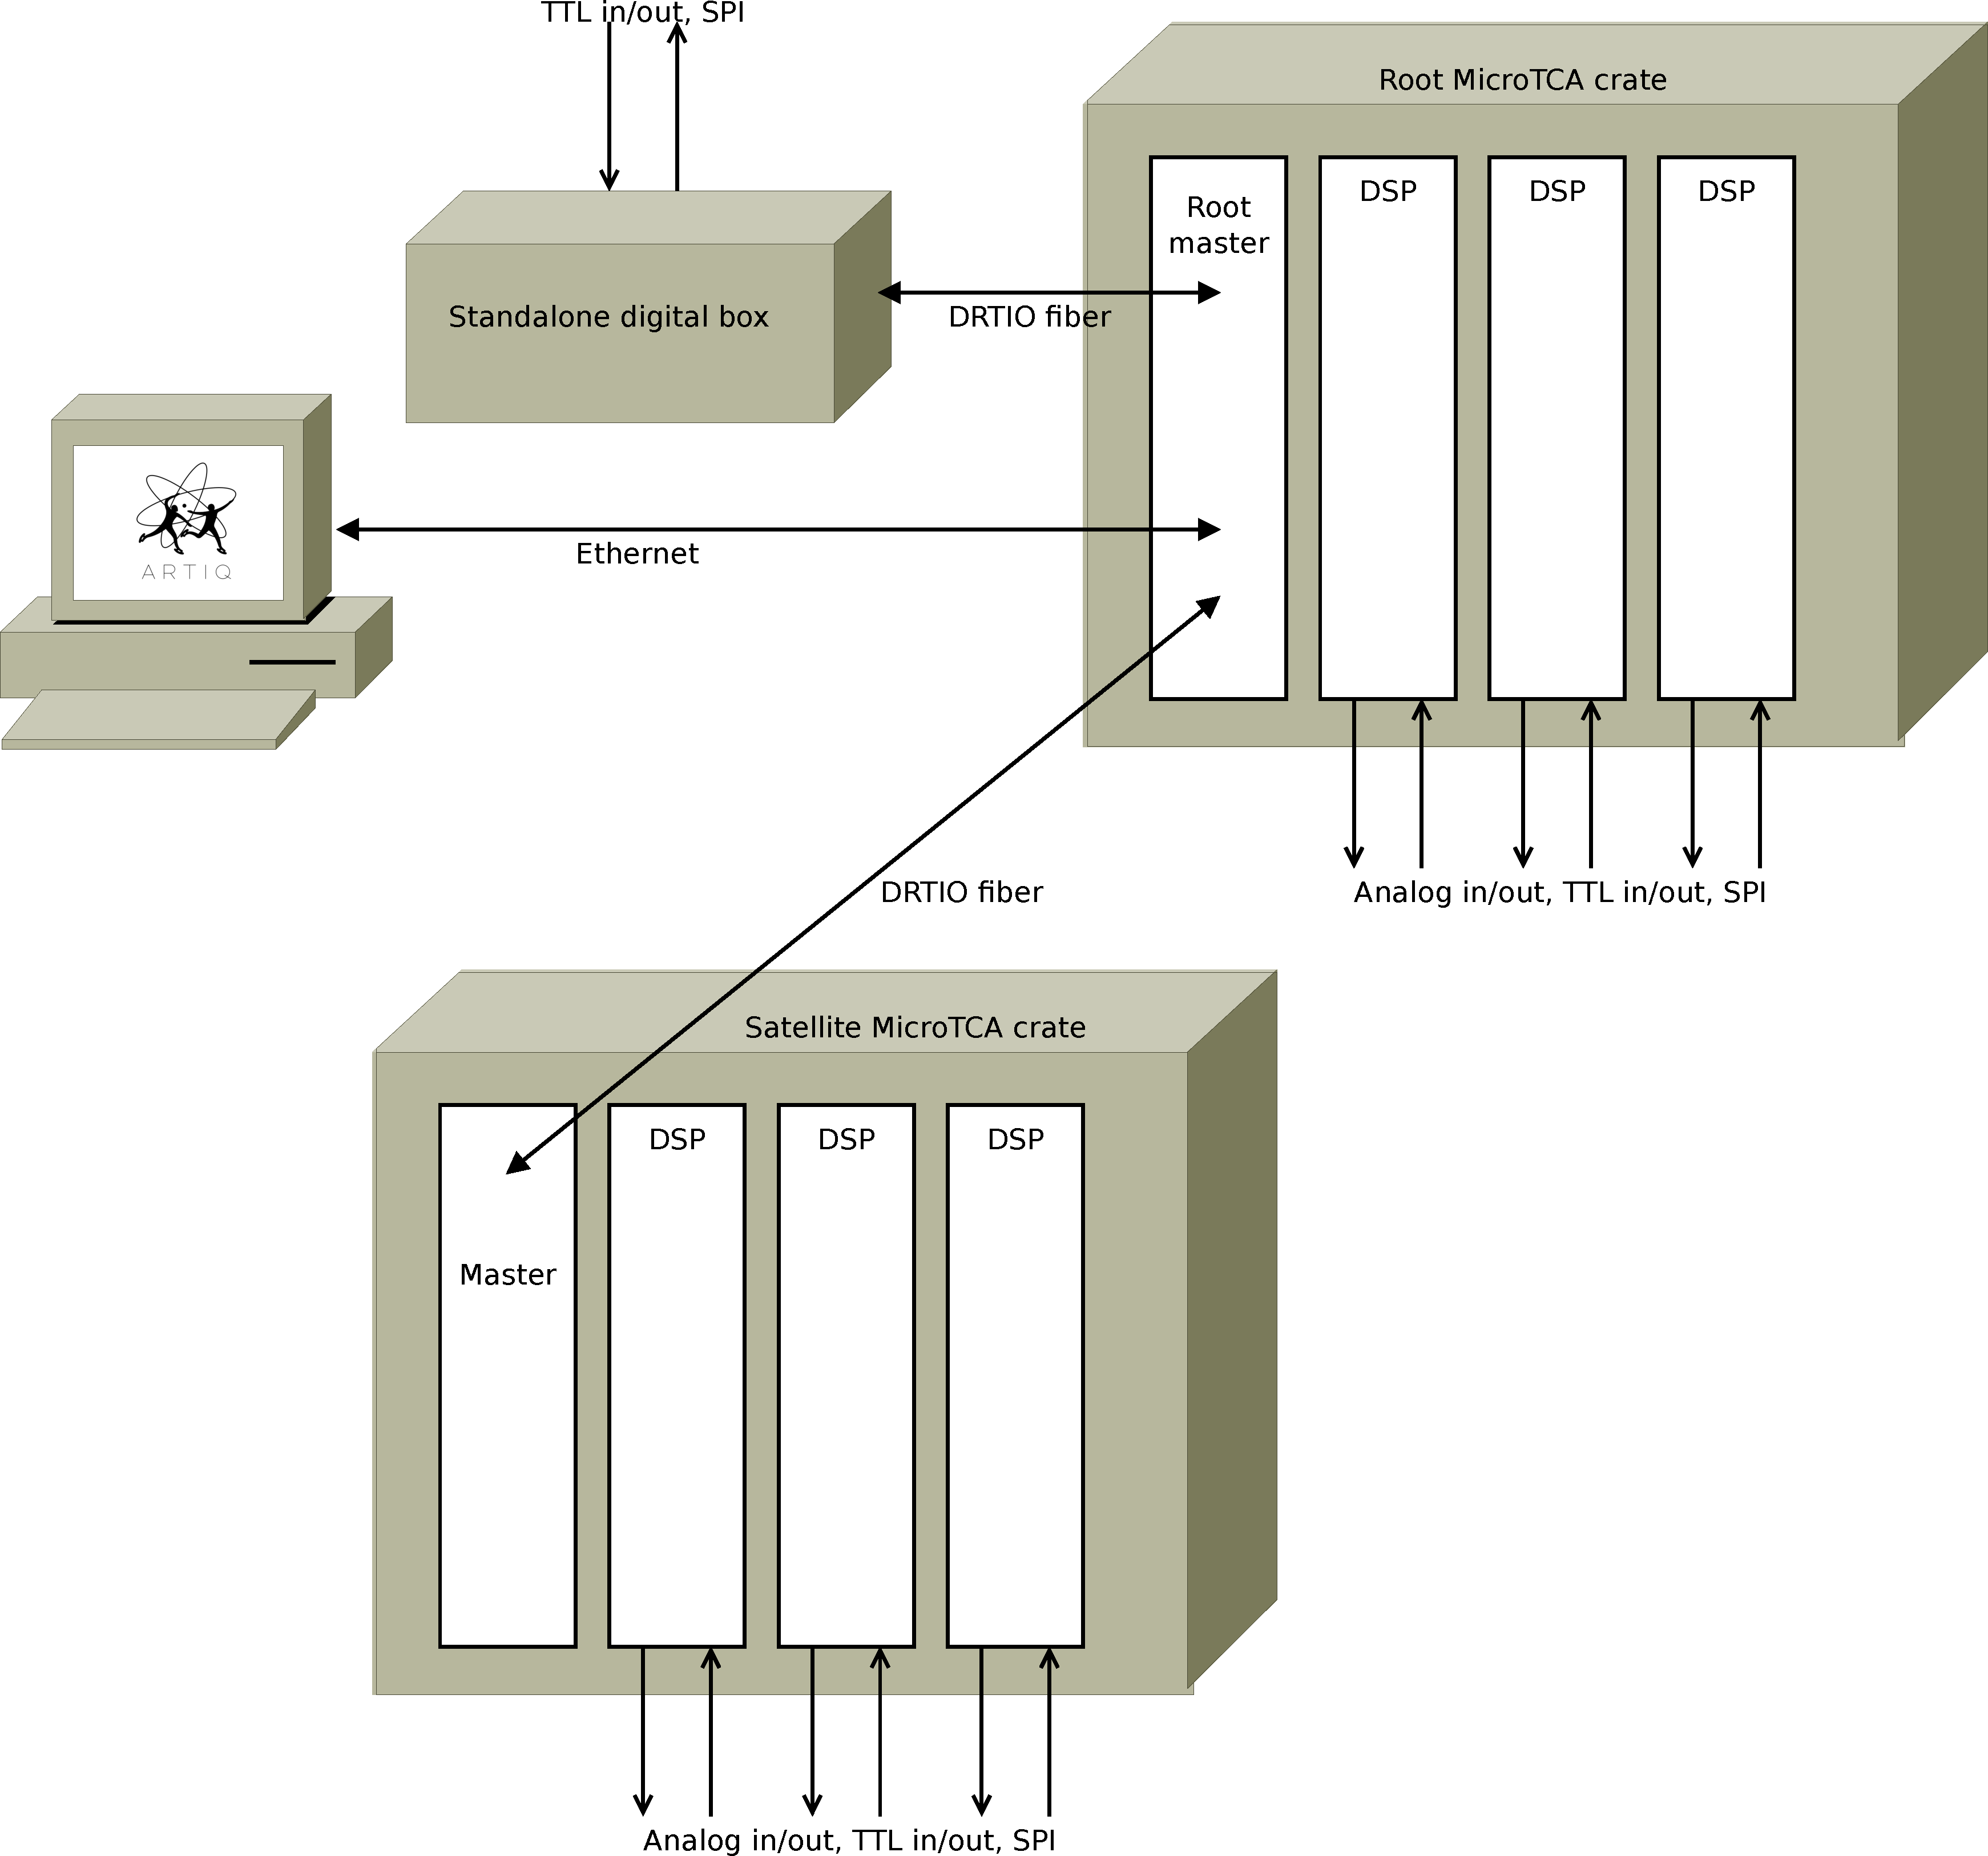
\includegraphics[width=\textwidth]{overview.pdf}

\section{MicroTCA crates}
The crates are compatible with the MicroTCA standard, and contain a power supply, cooling fans, a backplane (star topology), AMCs and MCH. In order to save space, and to keep all connectors on the same side, RTMs (MicroTCA.4) are not used and the crate should be chosen accordingly.

MicroTCA specifies a complicated ``IPMI'' management system. For compatibility reasons with other MicroTCA systems, the necessary hardware (a microcontroller circuit) should be present on the AMCs, but IPMI should otherwise be ignored as much as possible e.g.\ by keeping the power supplies on at all times.

To upgrade the gateware/runtime, firmware binaries are sent over the fiber or Ethernet for the FPGAs to write into their flash and reboot themselves, which is relatively simple and does not require additional hardware.

\section{Metlino boards}
A Metlino board is a double-width MicroTCA Carrier Hub (MCH) that:
\begin{itemize}
\item distributes DRTIO commands to the other cards in the crate over the MicroTCA backplane (star topology)
\item distributes DRTIO commands to other crates
\item receives commands from another Metlino board or the control PC
\end{itemize}

It has TBD SFPs on its front panel that are used for connecting to other devices (another Metlino board, TTL box, ...) over raw fiber optics, or to the control PC over Ethernet. The same fiber optic links may also be used for time transfer.

Metlino cards also have a digital I/O connector (VHDCI) on their front panel, that can be used to implement TTLs with little additional hardware.

A special Metlino board is the root master, which has the same role as the current core device in ARTIQ. It uses the same hardware as other master boards, but one of its SFPs is populated with a Ethernet PHY that is used to communicate with the control PC.

Metlino boards includes clock recovery and cleanup circuitry, and can be used to clock the other boards in the crate. A Metlino board also includes a SMA clock input connector on its front panel, in case the clock recovered from SFP is not of sufficient quality for the application, and for clocking the root master.

The FPGA used in Metlino boards is TBD (Kintex-7 or Zynq Ultrascale+, needs testing of Zynq).

\section{Sayma boards}
The Sayma boards are double-width AMC cards that contain a FPGA, fast SDRAM (e.g.\ DDR3 or DDR4), and which are typically used to generate and process RF signals via high-speed DACs and ADCs.

The ADCs and DACs are mounted on external FMC cards called ``RF daughter cards''. The Sayma cards have two identical FMC slots, one may be used for transmitting signals (DACs) and one for receiving (ADCs).

The FMC connectors use the LPC pin assignments, plus 8 transceivers using the HPC pin assignments. Some HPC ground pins are repurposed to provide +5V, -5V, +15V and -15V to the FMC mezzanine cards. The use of ground pins (and current limits on the power supplies) prevents damage when incorrect FMC mezzanines are plugged. The Sayma cards also have jumpers that disable those power supplies so that regular LPC + HPC transceivers FMC cards can be plugged.

Sayma boards receive high level DRTIO commands from the backplane, and synthesize, buffer or process waveforms using their FPGA and SDRAM.

The FPGA used in Sayma boards is XC7K325T (resource requirements: 28 kLUT, 14\% of the chip per DAC IQ channel pair at 1.25 GS/s, 16 bit). DRTIO is implemented over IOSERDES as all the transceivers are used for the FMCs.

\section{RF daughter cards}
\subsection{Commonalities}
RF daughter cards are FMC cards that are mounted on Sayma carriers.

Output cards contain one JESD204 multi-channel high-speed DAC (AD9154, 4 channels in total).

Input cards contain one JESD204 multi-channel ADC (AD9656, 4 channels in total).

The synchronization signals of the DACs and ADCs must be accessible to the FPGA to support synchronization across multiple cards.

All output cards can be clocked from the FMC connector (which the DSP card can connect to a backplane clock, potentially through a PLL that upconverts it from 10-100MHz, TBD), and from a dedicated SMA connector on their front panel (selectable by jumper, solder, or digitally controlled switch). High-quality clock distribution systems using semi-rigid coaxial cables can be used for particularly sensitive applications. The clock connector can also be used to experiment with different clocking systems. The output cards thus have 5 SMA connectors on the front panel, which is the maximum number that fit in that limited space.

Input cards may omit the external clock connector, as the ADCs are slower and the applications are less sensitive to clock noise when acquiring signals.

Input and output cards come in simple versions that contain only the basic circuitry plus an area that can receive a user-designed castellated module. Footprints for the castellated modules may be similar to those used by Marki Microwave.

\subsection{Karabash simple output card}
The four DAC channels are connected to pads that can receive a castellated prototyping module. The output card also has four SMA connectors on its front panel (in addition to the clock connector), with traces to the castellated module.

As part of this project, we shall provide a pass-through castellated module that connects the DACs directly to the SMA connectors.

\subsection{Ulvidy low frequency output card}
Signal bandwidth of a few MHz, swinging between +/- 10 V or so, suitable for ion trap transport waveforms or various DC or quasi-DC bias signals in general applications. This would involve op amps/instrumentation amps running off +/- 15V supplies in a similar configuration to the current PDQ output stages. Footprints for discrete component filters both before and after the amplifiers should be included.

\subsection{Argayash RF output card}
For synthesis of tones from a few MHz out to about 3.3 GHz, suitable for AOM drive, or Be\textsuperscript{+}, Mg\textsuperscript{+}, Ca\textsuperscript{+} and NV center microwave transitions. This would involve a set of filters (common footprint, stuff boards with different cutoff parts to define band of interest -- these can be left open for users, or we can choose one or two basic frequency sets and they can run their own custom assembly order from the fab/layout docs if they want something different, TBD) followed by an RF amplifier stage (ERA-4SM is a good broadband low-phase-noise selection), a digital step attenuator, and a fast high-isolation RF switch.

\subsection{Tatysh upconverting output card}
For synthesis of tones beyond about 3.3 GHz, suitable for Yb\textsuperscript{+} or superconducting qubit microwave transitions. The board would have an input connector for an externally generated microwave carrier, split and sent to the LO ports of a set of mixers/modulators. We should decide (TBD) if these needs to be IQ mixers or if regular mixers are sufficient. There will be filters (again, common footprint for a choice of frequencies) between the DAC outputs and mixer IF ports. Each mixer RF port will be followed by an amplifier, a digital step attenuator, and a fast high-isolation RF switch.

\subsection{Allaki simple input card}
The four ADC input channels go through a signal conditioner (amplifiers/attenuators) configurable by the FPGA (variable gain) before they reach a castellated module. The card has four SMA connectors on the front panel that are connected to the castellated module.

As part of this project, we shall provide a pass-through castellated module that connects the signal conditioner directly to the SMA connectors.

\section{Kasli boxes}
The Kasli boxes receive DRTIO commands (and optionally time) over a SFP and fiber connected to a master card, and generate and receive TTL pulses and digitally control devices such as SPI integrated circuits. They have TBD SMA connectors and TBD RJ45 connectors that can be connected to e.g.\ SPI devices. They contain their own power supply.

The Kasli boxes also have a dedicated clock input SMA connector, that can override the clock recovered from the SFP.

For convenience, the boxes also contain one AD5370 SPI DAC with its 40 channels connected to a D-sub connector (e.g.\ DD-50).

The FPGA used in Kasli boxes is XC6SLX45T.

\end{document}
